%\begin{savequote}[8cm]
%Simplicity is prerequisite for reliability.
%  \qauthor{--- Edsger W. Dijkstra}
%\end{savequote}

\chapter{\label{ch:polycubes_intro}An introduction to modular assembly}

\minitoc

From the start, the field of structural DNA nanotechnology has been interested in modular assemblies, although initially in the form of infinite and uniform crystal structures. In fact, Professor Ned Seeman was inspired to pioneer the field after seeing the woodcut \emph{Depth} by M.C. Escher, where fish are depicted organised into a neat crystalline structure \cite{seeman_2016}.

However, components that self-assemble into chrystals can also assemble bounded structures, if only a way can be found to make them self-limiting. The question is how many unique components would be required, relating to the complexity question introduced in Section~\ref{sec:AIT}.

This chapter will provide an overview of the background of self-assembled multicomponent structures, both bounded and unbounded, starting with experimental results of ever-increasing size and followed by a selection of theoretical models.

\section{Experimental applications} \label{sec:experimental_appl}
From small tiles made from a handful of strands to megadalton-scale structures made from multiple origami designs, modular self-assembly has seen considerable experimental research. This section provides a quick overview to some results of particular interest to the polycube model presented in Chapter~\ref{ch:polycubes1}.

\subsection{DNA tiles}
\label{sec:dna_tiles_bricks}
Following early nucleic acid multi-arm junctions and lattices suggested by Seeman \cite{seeman1982nucleic}, Winfree \cite{winfree1998algorithmic, winfree1998design} used double-crossover (DX) motifs, shown in Figure~\ref{fig:dna_tiles}.a, to self-assemble 2D DNA crystals. As can be seen in figure~\ref{fig:dna_tiles}.b, the lattices could be made with varying complexity, exemplified using either two or four different species of tiles.
% Tiles: https://www.nature.com/articles/28998

\begin{figure}[h]
  \centering
  \begin{overpic}[width=0.7\textwidth]{figures/dna_tiles.png}
    \put(0,450){a)}
    \put(0,240){b)}
  \end{overpic}
  \caption{DX tiles forming 2D lattices, adapted from \cite{winfree1998design}. a) Examples of DAO and DAE tile designs. b) Lattices made from two and four tile species respectively.}
  \label{fig:dna_tiles}
\end{figure}


\subsection{DNA bricks}
% Bricks: https://www.nature.com/articles/nature24648

A three-dimensional DNA ``canvas'' was created in 2017 by Ong et al. \cite{ong2017programmable}, called \emph{DNA bricks}. Structures are assembled from up to about 30,000 unique components, as seen in Figure~\ref{fig:dna_bricks}. Since each component consists of a unique strand, custom shapes can be ``sculpted'' by leaving out the voxels (3D pixels) not required.

\begin{figure}[h]
  \centering
  \begin{overpic}[width=\textwidth]{figures/dna_bricks.png}
    \put(0,350){a)}
    \put(450,350){b)}
    \put(450,120){c)}
  \end{overpic}
  \caption{DNA bricks, adapted from \cite{ong2017programmable}. a) DNA brick structure, where each of the up to 30'000 unique components is a 52 nucleotide DNA strand. The strands connect through a 13 base pair complementary domain at a 90 degree dihedral angle. b) A cuboid, here shown with 10,000 components, corresponds to a 20,000 voxel canvas. c) Approximating the shape of a teddy bear by removing a subset of the voxels from the canvas.}
  \label{fig:dna_bricks}
\end{figure}

\subsection{RNA tiles}
%https://www.science.org/doi/abs/10.1126/science.1253920 
As already covered in Section~\ref{sec:RNA_design}, it is possible to co-transcriptionally fold \emph{RNA origami} \cite{geary2014single}. This was first shown in 2014 by Geary et al., who folded RNA tiles that connect through complementary 120-degree kissing loop interactions, as seen in Figure~\ref{fig:rna_tiles}, forming a hexagonal lattice.

\begin{figure}[h]
  \centering
  \begin{overpic}[width=\textwidth]{figures/rna_tiles.jpeg}
      \put(0,300){a)}
      \put(320,300){b)}
      \put(750,300){c)}
  \end{overpic}
  \caption{Co-transcriptional folding RNA origami tiles, adapted from \cite{geary2014single}. The tiles connect through 120-degree kissing loop interactions, forming a hexagonal lattice. a) Detailed scematic of the four-helix 4H-AO tile. b) Co-transcriptional folding, where the RNA tile folds as it is transcribed from a DNA template. c) Hexagonal lattice formed by folded tiles.}
  \label{fig:rna_tiles}
\end{figure}

\subsection{Finite DNA origami arrays}\label{sec:origamiArrays}
% https://www.nature.com/articles/nature24655

In 2017, Tikhomirov et al.\cite{tikhomirov2017fractal, tikhomirov2017programmable} used the DNA origami technique to demonstrate two-dimensional patterns assembled on the micrometre-scale using square tiles where each tile was a complete origami, as seen in Figure~\ref{fig:origamiArrays}. The tiles connect to each other through complementary single-stranded overhangs on their edges.

The patterns could either be hierarchically assembled from unique tiles \cite{tikhomirov2017fractal}, or assembled into random patterns from a small number of tile types \cite{tikhomirov2017programmable}. The binding strength could be calibrated using a variable amount of edge overhangs, as seen in Figure~\ref{fig:origamiArrays}.b). Arrays up to \(8 \times 8\) tiles were successfully produced, although larger arrays had a much smaller yield (Figure~\ref{fig:origamiArrays}.c).

While the random tilings were generally unbounded, Tikhomirov et al. also showed how to program a finite grid (see Figure~\ref{fig:origamiArrays}.d).

\begin{figure}[h]
  \centering
  \begin{overpic}[width=\textwidth]{figures/monalisa_tiles.png}
    \put(-20,580){a)}
    \put(200,580){b)}
    \put(-20,150){c)}
    \put(600,580){d)}
  \end{overpic}
  \caption{DNA origami arrays, adapted from \cite{tikhomirov2017fractal, tikhomirov2017programmable}. a) Strand-level diagram of a \(12 \times 12\) version of the the origami tile (actual size is \(22 \times 22\) helices). b) \(4 \times 4\) tile ``Mona Lisa'' pattern. c) AFM image of patterned assemblies of different sizes (left) with their respective yields (right). d) Abstract design diagrams (left) and AFM images (right) of finite origami arrays, designed to different sizes \cite{tikhomirov2017programmable}.}
  \label{fig:origamiArrays}
\end{figure}

\subsection{Shape-complementary origami}
% 2D https://www.nature.com/articles/nchem.1070
% 3D https://science.sciencemag.org/content/347/6229/1446.abstract

% Huge https://www.nature.com/articles/s41563-021-01020-4

Also, in 2017, Wagenbauer et al. \cite{wagenbauer2017gigadalton} used shape-complementarity to assemble DNA origami components into three-dimensional polyhedral shapes up to 450 nanometers in diameter. Later, in 2021, Sigl et al. assembled large shells from shape-complementary origami triangles, as seen in Figure~\ref{fig:shape-complementarity}. The triangular sides attach through helix protrusions and indentations of complementary shape, as seen in figure~\ref{fig:shape-complementarity}.a), binding together through blunt-end stacking interactions, a method first shown by Woo et al. \cite{woo2011programmable}.

\begin{figure}[h]
  \centering
  \begin{overpic}[width=\textwidth]{figures/icosahedral_shell.png}
    \put(0,320){a)}
    \put(620,320){b)}
  \end{overpic}
  \caption{Shape-complementary triangles assembling polyhedral shells. Adapted from \cite{sigl2021programmable}. a) Polyhedral shell design for T=9. \(N\) is the triangulation number (the number of unique edges required for assembly), \(\alpha\) is the bevel angle of the triangle sides, and \(N\) is the number of triangles required for a full shell. b) Cryo-EM reconstruction of an assembled T=4 icosahedral shell.}
  \label{fig:shape-complementarity}
\end{figure}


\subsection{DNA origami nanochambers}
% https://pubs.acs.org/doi/full/10.1021/jacs.0c07263

In 2020, Lin et al.\cite{nano-chambers_lin2020} presented cubic DNA origami ``nanochambers''. The chambers have sticky-end overhangs on every side of the cube, allowing it to assemble in 1D, 2Dm and 3D, as can be seen in Figure~\ref{fig:nanochambers}. However, since the shape is only rotationally symmetric around the z-axis, the assembly is a limited subset of the polycube model described in Chapter~\ref{ch:polycubes1}. 

\begin{figure}[h!]
  \centering
  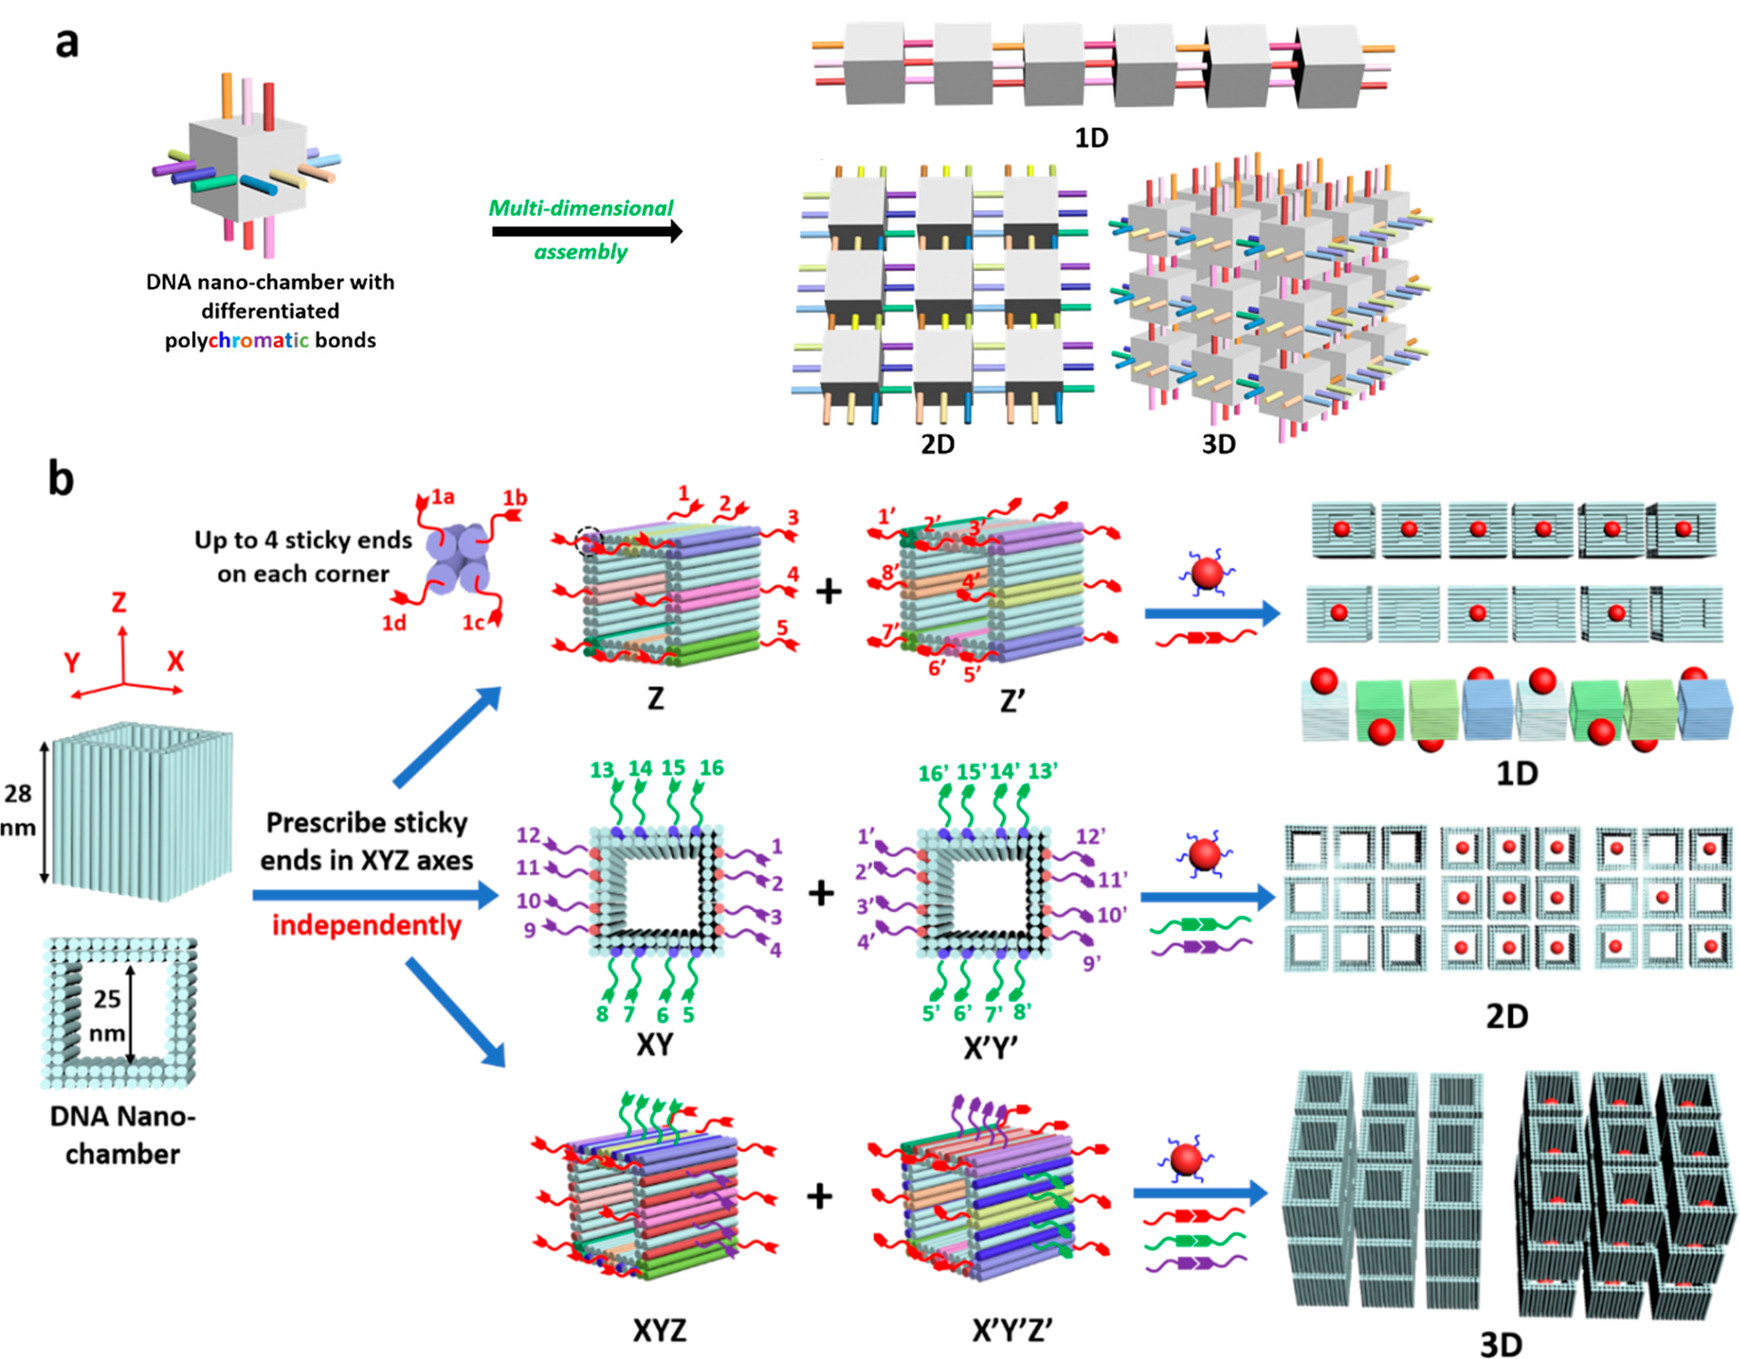
\includegraphics{figures/nanochambers2.jpeg}
  \caption{DNA origami nanochambers, adapted from \cite{nano-chambers_lin2020}. a) Concept illustration, where building blocks with \emph{polychromatic} bonds (differentiated though different single-stranded sequences), assemble into 1D, 2D, and 3D structures. b) Schematic of DNA nanochamber programmable assembly, showing sticky end overhangs applied in 1D, 2D, and 3D assemblies.}
  \label{fig:nanochambers}
\end{figure}

\subsection{Octahedral DNA origami frames}
In 2020, Wang et al. \cite{tian_octahedra2020} showed how octahedral DNA origami frames could be used as building blocks in limited and unlimited programmed assemblies, as seen in Figure~\ref{fig:tian_octahedra}. Using sticky-end overhangs at the octahedral vertices, the building blocks have the connectivity, as well as the rotational symmetry, of a cube.

Due to the flexibility of the single-stranded connections, the connections are less torsionally rigid than assumed in the polycube model, later described in Chapter~\ref{ch:polycubes1}. However, as can be seen in Figure~\ref{fig:tian_octahedra}, shapes such as the cube can still be assembled with good yield.

% https://onlinelibrary.wiley.com/doi/abs/10.1002/anie.201913958

\begin{figure}[!h]
  \centering
  \begin{overpic}[width=\textwidth]{figures/tian.jpg}
    \put(0,480){a)}
    \put(280,480){b)}
    \put(670,480){c)}
  \end{overpic}
  \caption{Octahedral DNA origami frames, adapted from \cite{tian_octahedra2020}. a) Two octahedra with complementary sticky ends binding together to form a dimer. The edges consist of six-helix bundles. b) nanoclusters assembled from different sets of building blocks. c) \(2 \times 2 \times 2 \) cube nano cluster (top) and histogram of the mass fraction, where the intended design of eight components per cluster is the most common.}
  \label{fig:tian_octahedra}
\end{figure}


\section{Modular assembly models}
It would be computationally unreasonable to simulate module assembly at the level of individual nucleotides. A simpler approach is to use an abstract model to predict the assembly process with the modules treated as rigid bodies or discrete tiles. This section will present earlier such models as a background to my own polycube model, described in Chapter~\ref{ch:polycubes1}.

\subsection{Wang tiles}
Introduced by Hao Wang in 1961 \cite{wang1961proving}, so-called \emph{Wang tiles} are square tiles with a colour on each of their four edges. Without rotating or reflecting the tiles, they assemble so that adjacent edges have the same colour.

%\begin{figure}[h]
 % \centering\includesvg[width=0.5\textwidth]{figures/Wang_11_tiles.svg}
 % \caption{Wang tiles}
%\end{figure}

The DNA tiles by Winfree et al. \cite{winfree1998design}, presented in Section~\ref{sec:dna_tiles_bricks}, behave like Wang tiles by design and do not allow rotations or reflections. Winfree investigated the possibility of using such tiles for computation \cite{winfree1998algorithmic}, which led to aTAM: the algorithmic Tile Assembly Model.

\subsection{The algorithmic tile assembly model}
\label{sec:atam}
% David Doty overview: https://cacm.acm.org/magazines/2012/12/157881-theory-of-algorithmic-self-assembly/fulltext

% Molecular algorithms https://www.nature.com/articles/s41586-019-1014-9

The algorithmic Tile Assembly Model (aTAM), shown in Figure~\ref{fig:atam}, models the dynamic behaviour of the double crossover DNA tiles introduced by Winfree et al. \cite{winfree1998design}. Each tile has four patches, one on each edge, corresponding to the four single-stranded regions of the DNA tile. Furthermore, the patches can have different strengths, with a global temperature variable determining the total connection strength required for a tile to attach \cite{doty2012theory}.

In the example seen in Figure~\ref{fig:atam}, the pattern grows from the initial bottom-right seed into the blue horizontal bottom row and the rightmost vertical column. This is because these tiles have ``strength-2'' glues with enough binding strength to attach by themselves \cite{doty2012theory}. The additional tiles have weaker ``strength-1'' glues (illustrated as thinner black connectors), so they need at least two complementary patches to achieve the binding strength threshold (temperature).

Because of this so-called co-operative binding, the tiles can be seen as logic gates performing computation; given the bottom and right patches as input bits, the matching tile attaches and produces two computed output bits (top and left).

% DX array https://www.nature.com/articles/28998


\begin{figure}[h]
  \centering\includesvg[width=\textwidth]{figures/atam.svg}
  \caption{Algorithmic self-assembly of a Sierpiński triangle. Adapted from \cite{doty2017}. A tile set (right) grows from an initial seed by co-operatively attaching self-complementary edges (without rotation). The \(0\) and \(0\) ``glues'' are weaker and require two matching bonds to attach (co-operative binding), compared to the \(W\) (west) and \(N\) (north) glues that are strong enough to bind alone.}
  \label{fig:atam}
\end{figure}

\subsection{The polyomino model}\label{sec:polyomino}

The main inspiration for the \emph{polycube} model presented in Chapter~\ref{ch:polycubes1} is the polyomino model \cite{ahnert2010self, johnston2011evolutionary}. The 2D model is similar in assembly to the later experimental micro-meter scale tile designs by Tikhomirov \cite{tikhomirov2017programmable} shown in Figure~\ref{fig:origamiArrays}.d). Compared to the abstract tile assembly model described in Section~\ref{sec:atam}, polyomino tiles are allowed to rotate, creating further possibilities for symmetries. Also, the edge binding is not self-complementary, with complementary colour pairs used instead. Finally, polyominoes have a constant binding strength (in other words, a temperature-1 model), avoiding co-operative binding.

See Figure~\ref{fig:polyominoes} for an illustration of the model, where an input \emph{genotype} genotype (describing the four possible tile types) is mapped into an assembled output polyomino by stochastically growing the shape from an initial seed. The growth stops if, as in the example in Figure~\ref{fig:polyominoes}, no more tiles can attach (since the colour \(0\) does not bind to anything). If the growth is infinite, the genotype is called \emph{unbounded}. A genotype is considered deterministic if it assembles the same phenotype polyomino every time. Only bounded and deterministic genotypes are considered valid inputs.

\begin{figure}[h]
    \centering
    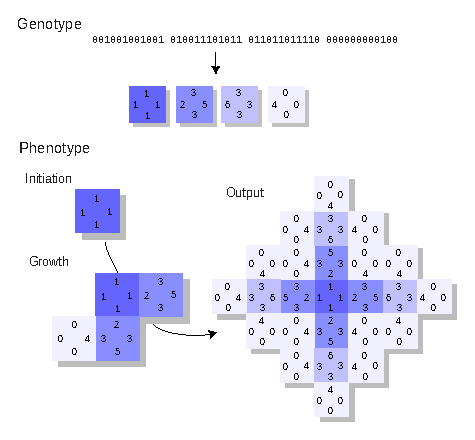
\includegraphics[width=0.6\textwidth]{figures/polyominoes.eps}
    \caption{Illustration of the polyomino assembly model, adapted from \cite{johnston2011evolutionary}. A \emph{genotype}, in the form of a ruleset of possible tiles, encodes for a polyomino \emph{phenotype}, grown stochastically from an initial seed tile.}
    \label{fig:polyominoes}
\end{figure}

In 2021, evolutionary runs of polyominoes were shown to have a clear bias toward structures with low complexity and high symmetry \cite{johnston2021}. See Figure~\ref{fig:polyomino_symmetries}, where the frequency of protein complexes and polyominoes are compared to their complexity. To be clear, the number of interface types required (number of patch colours in the polyomino case) is used as a proxy measure for the Komologrov complexity of the structure (see Section~\ref{sec:AIT}).

The fitness of the structures only depended on their size (16-mers had the highest fitness), so the simplicity was not selected for but is rather a property of the mapping. This is in line with the Algorithmic Information Theory arguments made by Dingle et al. \cite{dingle2018input}, who showed the same simplicity bias for a set of various input-output maps.

\begin{figure}[h]
  \centering
  \begin{overpic}[width=0.9\textwidth]{figures/polyomino_symm_and_simpl.eps}
    \put(0,750){a)}
    \put(520,750){b)}
    \put(0,590){c)}
    \put(520,590){d)}
  \end{overpic}
  \caption{Frequent symmetry and simplicity through evolution, adapted from \cite{johnston2021}. Both protein complexes (a) and polyominoes (b) self-assemble from individual units. c) Frequency of 6-mer protein complex topologies in the protein data bank, versus their complexity (measured as the number of interface types) d) Frequency versus complexity of polyominoes found in evolutionary runs with a fitness function seeking 16-mers.}
  \label{fig:polyomino_symmetries}
\end{figure}


\subsection{Patchy particle simulation}
\label{sec:patchy_particles}

Besides discrete tile models, self-assembly can also be modelled using Molecular Dynamics simulations of rigid-body spheres called \emph{patchy particles}. Each particle has a number of patches that bind when they come in contact with another complementary patch.

One such patchy particle simulator is included as part of the oxDNA package \cite{rovigatti2015comparison}. It was, for example, used by Romano et al., as seen in Figure~\ref{fig:patchy_particles}, to verify the patchy interactions designed by their SAT-solver method \cite{romano2020designing}.


\begin{figure}[h]
  \centering
  \begin{overpic}[width=\textwidth]{figures/patchy_particles.png}
    \put(0,310){a)}
    \put(280,310){b)}
    \put(650,310){c)}
  \end{overpic}
  \caption{Patchy particle simulation, adapted from \cite{romano2020designing}. a) The unit cell of a tetrastack lattice build with patchy particles. b) Simulation snapshot of a forming tetrastack lattice. Note the free-flowing particles that have not yet attached the growing latttice they surround. c) Tetrastack particle energy plotted over simulation time for different temperatures. Sudden drops in energy correspond to nucleation events (where the lattices start forming).}
  \label{fig:patchy_particles}
\end{figure}

In this thesis, the same patchy particle model is used to produce the results seen in Chapter~\ref{ch:polycubes2}. However, to account for the polycube requirement of patch orientation alignment, the model has been modified to include torsional interactions.